% !TeX spellcheck = en_US
\usetikzlibrary{calc,arrows.meta,positioning}
\tikzset{
    every node/.style={font=\sffamily\small},
    main node/.style={shape=rectangle, rounded corners,
    	draw, align=center,
    	top color=white, bottom color=blue!20},
    data node/.style={shape=rectangle,
    draw, align=center,
    top color=white, bottom color=red!20}
}

\begin{figure}
	\centering
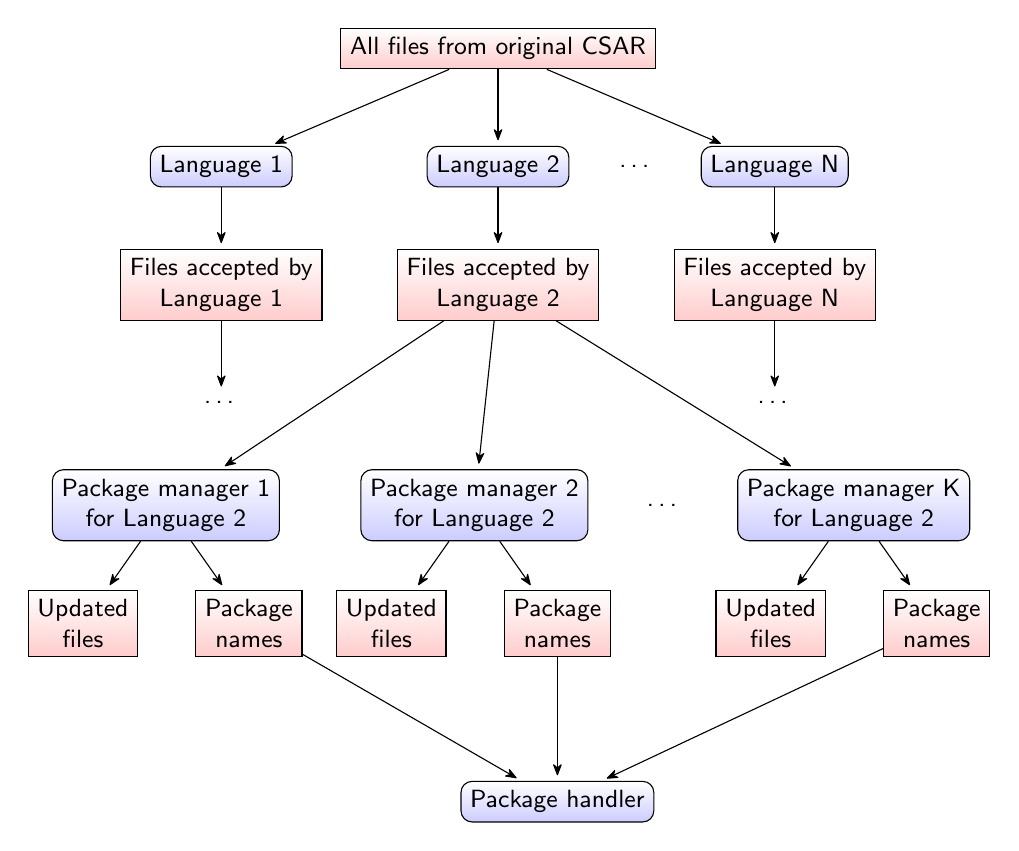
\begin{tikzpicture}[->,>={Stealth[round,sep]},shorten >=1pt,auto,level 1/.style={sibling distance=10em,node distance=25mm},
level 2/.style={sibling distance=8em,node distance=30mm},
level 3/.style={sibling distance=12em,node distance=30mm},
level 4/.style={sibling distance=6em,node distance=25mm},
level 5/.style={sibling distance=8em,node distance=25mm},
level 6/.style={sibling distance=8em,node distance=25mm}]
    \node[data node] (1)  {All files from original CSAR}
    child { node[main node](2) {Language 1} 
    	child { node[data node](21) {Files accepted by\\ Language 1} 
    		child { node {\ldots}}}}
	child { node[main node] (3) {Language 2}
		child { node[data node](31) {Files accepted by\\ Language 2} 
			child { node[main node, yshift=-13mm](32) {Package manager 1\\for Language 2} 
				child { node[data node](36) {Updated\\ files}}
				child { node[data node](37) {Package\\ names}}}
			child { node[main node, yshift=-13mm, xshift=-3mm](33) {Package manager 2\\for Language 2}
				child { node[data node](34) {Updated\\ files}}
				child { node[data node](35) {Package\\ names}}}
			child { node[main node, yshift=-13mm, xshift=+3mm](34) {Package manager K\\for Language 2}
				child { node[data node](38) {Updated\\ files}}
				child { node[data node](39) {Package\\ names}}}
			}
		}
    child { node[main node] (4) {Language N}
    	child { node[data node](41) {Files accepted by\\ Language N} 
    		child { node {\ldots}}}}
	;

	\node [main node,below, yshift=-20mm] at (35) (ph) {Package handler};
    \node at ($(3)!.5!(4)$) {\ldots};
    \node at ($(33)!.5!(34)$) {\ldots};
    \draw [->] (35) --(ph);
    \draw [->] (37) --(ph);
    \draw [->] (39) --(ph);
    
\end{tikzpicture} 
\caption{Data flow scheme between language modules, package manager modules and package handler.} 	\label{fig:lang_ph}
\end{figure}